\subsection{Panel właściciela siłowni}\label{subsec:panel-wasciciela-siowni}

{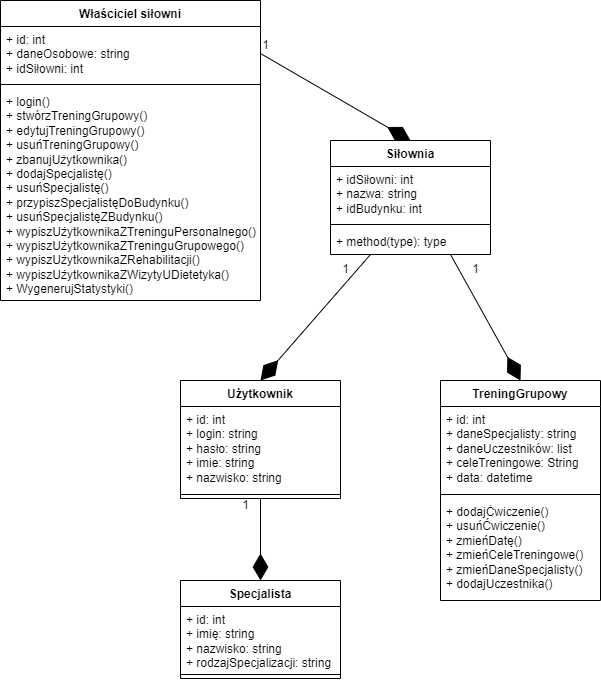
\includegraphics{diagrams/use_cases/wlasciciel_silowni}}

{\includegraphics{diagrams/use_cases/wlasciciel_silowni_hierarchy}}

\begin{enumerate}
\setcounter{enumi}{10}
\tightlist
\item
  {Stwórz trening grupowy}
\end{enumerate}

{~~~~~~~~}{Aktorzy biorący udział: Właściciel siłowni}

{~~~~~~~~Cel przypadku: Utworzenie treningu grupowego dla klientów.}

{~~~~~~~~Warunki początkowe: Właściciel siłowni jest zalogowany w
systemie i ma dostęp do panelu właściciela siłowni.}

{~~~~~~~~Warunki końcowe: Utworzony trening grupowy, który jest dostępny
dla użytkowników.}

{~~~~~~~~Główny ciąg zdarzeń:}

\begin{enumerate}
\tightlist
\item
  {Właściciel siłowni wybiera opcję "Tworzenie treningu grupowego".}
\item
  {System wyświetla formularz, w którym właściciel siłowni może
  wprowadzić informacje dotyczące treningu, takie jak:}
\end{enumerate}

\begin{itemize}
\tightlist
\item
  {Nazwa treningu}
\item
  {Data i godzina rozpoczęcia}
\item
  {Czas trwania treningu}
\item
  {Maksymalna liczba uczestników}
\item
  {Opis treningu (np. rodzaj ćwiczeń, poziom trudności itp.)}
\end{itemize}

\begin{enumerate}
\setcounter{enumi}{2}
\tightlist
\item
  {Użytkownik uzupełnia formularz i zapisuje trening.}
\item
  {System potwierdza utworzenie treningu i automatycznie dodaje go do
  harmonogramu zajęć w aplikacji siłowni.}
\end{enumerate}

{~~~~~~~~Alternatywne ciąg zdarzeń:}

\begin{itemize}
\tightlist
\item
  {Użytkownik nie posiada uprawnień właściciela siłowni.}
\end{itemize}

\begin{itemize}
\tightlist
\item
  {System wyświetla komunikat o braku uprawnień.}
\end{itemize}

\begin{itemize}
\tightlist
\item
  {Użytkownik wprowadził niepoprawne dane w formularzu.}
\end{itemize}

\begin{itemize}
\tightlist
\item
  {System wyświetla komunikat o niepoprawnie wprowadzonych danych i
  prosi o poprawienie danych.}
\end{itemize}

{}

\begin{enumerate}
\setcounter{enumi}{11}
\tightlist
\item
  {Edytuj trening grupowy}
\end{enumerate}

{Aktorzy biorący udział: Właściciel siłowni}

{~~~~~~~~Cel przypadku: Edycja treningu grupowego.}

{~~~~~~~~Warunki początkowe: Właściciel siłowni jest zalogowany w
systemie i ma dostęp do panelu właściciela siłowni.}

{~~~~~~~~Warunki końcowe: Zaktualizowany trening grupowy.}

{~~~~~~~~Główny ciąg zdarzeń:}

\begin{enumerate}
\tightlist
\item
  {Właściciel siłowni otwiera okno treningów grupowych.}
\item
  {Użytkownik wybiera odpowiedni trening grupowy.}
\item
  {System wyświetla dane treningu z możliwością edycji każdego pola.}
\item
  {Właściciel siłowni }{edytuje}{~i zapisuje dane.}
\item
  {~System potwierdza wprowadzone zmiany}
\end{enumerate}

{~~~~~~~~Alternatywny ciąg zdarzeń:}

\begin{itemize}
\tightlist
\item
  {Użytkownik nie posiada uprawnień właściciela siłowni.}
\end{itemize}

\begin{itemize}
\tightlist
\item
  {System wyświetla komunikat o braku uprawnień.}
\end{itemize}

\begin{itemize}
\tightlist
\item
  {Użytkownik wprowadził niepoprawne dane w formularzu.}
\end{itemize}

\begin{itemize}
\tightlist
\item
  {System wyświetla komunikat o niepoprawnie wprowadzonych danych i
  prosi o poprawienie danych.}
\end{itemize}

\begin{itemize}
\tightlist
\item
  {Użytkownik nie wprowadził zmian.}
\end{itemize}

{\hfill\break
}

\begin{enumerate}
\setcounter{enumi}{12}
\tightlist
\item
  {Usuń trening grupowy}
\end{enumerate}

{Aktorzy biorący udział: Właściciel siłowni}

{~~~~~~~~Cel przypadku: Usunięcie w systemie treningu grupowego.}

{~~~~~~~~Warunki początkowe: Właściciel siłowni jest zalogowany w
systemie i ma dostęp do panelu właściciela siłowni.}

{~~~~~~~~Warunki końcowe: Trening grupowy został usunięty.}

{~~~~~~~~Główny ciąg zdarzeń:}

\begin{enumerate}
\tightlist
\item
  {Właściciel siłowni otwiera okno treningów grupowych.}
\item
  {Użytkownik wybiera odpowiedni trening.}
\item
  {Właściciel siłowni wybiera opcję ``Usuń'' i potwierdza.}
\item
  {System potwierdza usunięcie treningu grupowego.}
\end{enumerate}

{~~~~~~~~Alternatywny ciąg zdarzeń:}

\begin{itemize}
\tightlist
\item
  {Użytkownik nie posiada uprawnień właściciela siłowni.}
\end{itemize}

\begin{itemize}
\tightlist
\item
  {System wyświetla komunikat o braku uprawnień.}
\end{itemize}

\begin{itemize}
\tightlist
\item
  {Brak treningów grupowych.}
\end{itemize}

\begin{itemize}
\tightlist
\item
  {System wyświetla komunikat o braku treningów grupowych.}
\end{itemize}

\begin{itemize}
\tightlist
\item
  {Właściciel siłowni nie potwierdził usunięcia.\\
  }
\end{itemize}

\begin{enumerate}
\setcounter{enumi}{13}
\tightlist
\item
  {Zbanuj użytkownika}
\end{enumerate}

{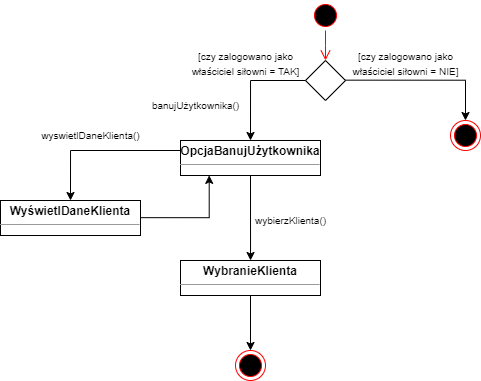
\includegraphics{diagrams/state/zbanuj_uzytkownika}}

{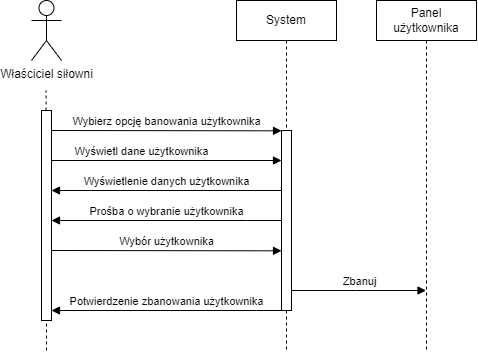
\includegraphics{diagrams/sequence/zbanuj_uzytkownika}}

{Aktorzy biorący udział: Właściciel siłowni}

{~~~~~~~~Cel przypadku: Zbanowanie użytkownika.}

{~~~~~~~~Warunki początkowe: Właściciel siłowni jest zalogowany w
systemie i ma dostęp do panelu właściciela siłowni.}

{~~~~~~~~Warunki końcowe: Wybrany użytkownik został zbanowany w
systemie.}

{~~~~~~~~Główny ciąg zdarzeń:}

\begin{enumerate}
\tightlist
\item
  {Właściciel siłowni otwiera listę użytkowników swojej siłowni.}
\item
  {Użytkownik wybiera osobę którą chce zbanować i potwierdza.}
\item
  {System zwraca komunikat potwierdzający zbanowanie użytkownika.}
\end{enumerate}

{~~~~~~~~Alternatywny ciąg zdarzeń:}

\begin{itemize}
\tightlist
\item
  {Użytkownik nie posiada uprawnień właściciela siłowni.}
\end{itemize}

\begin{itemize}
\tightlist
\item
  {System wyświetla komunikat o braku uprawnień.}
\end{itemize}

\begin{itemize}
\tightlist
\item
  {Brak użytkowników siłowni.}
\end{itemize}

\begin{itemize}
\tightlist
\item
  {System wyświetla komunikat o braku użytkowników.}
\end{itemize}

\begin{itemize}
\tightlist
\item
  {Właściciel siłowni nie potwierdził zbanowania.\\
  }
\end{itemize}

{}

{}

{}

{}

{}

{}

{}

\begin{enumerate}
\setcounter{enumi}{14}
\tightlist
\item
  {Dodaj specjalistę}
\end{enumerate}

{Aktorzy biorący udział: Właściciel siłowni}

{~~~~~~~~Cel przypadku: Dodanie w systemie specjalisty}

{~~~~~~~~Warunki początkowe: Właściciel siłowni jest zalogowany w
systemie i ma dostęp do panelu właściciela siłowni.}

{~~~~~~~~Warunki końcowe: Specjalista został dodany w systemie i jest
dostępny dla użytkowników.}

{~~~~~~~~Główny ciąg zdarzeń:}

\begin{enumerate}
\tightlist
\item
  {Właściciel siłowni otwiera okno ``Specjaliści''.}
\item
  {Użytkownik wybiera opcję ``Dodaj Specjalistę''.}
\item
  {System wyświetla formularz, w którym właściciel siłowni może
  wprowadzić informacje dotyczące specjalisty, takie jak:}
\end{enumerate}

\begin{itemize}
\tightlist
\item
  {Imię, Nazwisko}
\item
  {Numer telefonu}
\item
  {Rodzaj specjalisty}
\item
  {Godziny pracy}
\end{itemize}

\begin{enumerate}
\setcounter{enumi}{3}
\tightlist
\item
  {Użytkownik uzupełnia formularz i zapisuje w systemie.}
\item
  {System potwierdza dodanie specjalisty i dodaje go do listy dostępnych
  specjalistów dla użytkowników siłowni.}
\end{enumerate}

{~~~~~~~~Alternatywny ciąg zdarzeń:}

\begin{itemize}
\tightlist
\item
  {Użytkownik nie posiada uprawnień właściciela siłowni.}
\end{itemize}

\begin{itemize}
\tightlist
\item
  {System wyświetla komunikat o braku uprawnień.}
\end{itemize}

\begin{itemize}
\tightlist
\item
  {Właściciel siłowni otwiera listę użytkowników swojej siłowni.}
\end{itemize}

\begin{itemize}
\tightlist
\item
  {Wybiera odpowiedniego użytkownika i wybiera opcję ``Ustaw jako
  specjalistę''.}
\item
  {System wysyła zapytanie do użytkownika wraz z formularzem.}
\item
  {System potwierdza dodanie specjalisty i dodaje go do listy dostępnych
  specjalistów dla użytkowników siłowni.}
\end{itemize}

\begin{itemize}
\tightlist
\item
  {Użytkownik nie potwierdza zapytania/ nie wypełnia formularza.}
\item
  {Użytkownik/ Właściciel siłowni wprowadził niepoprawne dane w
  formularzu.}
\end{itemize}

\begin{itemize}
\tightlist
\item
  {System wyświetla komunikat o niepoprawnie wprowadzonych danych i
  prosi o poprawienie danych.\\
  }
\end{itemize}

\begin{enumerate}
\setcounter{enumi}{15}
\tightlist
\item
  {Edytuj specjalistę}
\end{enumerate}

{Aktorzy biorący udział: Właściciel siłowni}

{~~~~~~~~Cel przypadku: Edycja danych specjalisty.}

{~~~~~~~~Warunki początkowe: Właściciel siłowni jest zalogowany w
systemie i ma dostęp do panelu właściciela siłowni.}

{~~~~~~~~Warunki końcowe: Modyfikacja danych specjalisty.}

{~~~~~~~~Główny ciąg zdarzeń:}

\begin{enumerate}
\tightlist
\item
  {Właściciel siłowni otwiera okno ``Specjaliści''.}
\item
  {Użytkownik wybiera specjalistę docelowego.}
\item
  {Właściciel siłowni wybiera opcję ``Edytuj''.}
\item
  {Po edycji i danych i potwierdzeniu czynności system potwierdza
  zapisaną akcję.}
\item
  {Specjalista, którego były modyfikowane dane potwierdza wprowadzone
  zmiany.}
\item
  {Dane są zapisane w systemie i dostępne dla użytkowników.}
\end{enumerate}

{~~~~~~~~Alternatywny ciąg zdarzeń:}

\begin{itemize}
\tightlist
\item
  {Użytkownik nie posiada uprawnień właściciela siłowni.}
\end{itemize}

\begin{itemize}
\tightlist
\item
  {System wyświetla komunikat o braku uprawnień.}
\end{itemize}

\begin{itemize}
\tightlist
\item
  {Użytkownik wprowadził niepoprawne dane w formularzu.}
\end{itemize}

\begin{itemize}
\tightlist
\item
  {System wyświetla komunikat o niepoprawnie wprowadzonych danych i
  prosi o poprawienie danych.}
\end{itemize}

\begin{itemize}
\tightlist
\item
  {Użytkownik nie wprowadził zmian.}
\item
  {Dany specjalista nie potwierdził zmian}
\end{itemize}

{\hfill\break
}

\begin{enumerate}
\setcounter{enumi}{16}
\tightlist
\item
  {Usuń specjalistę}
\end{enumerate}

{Aktorzy biorący udział: Właściciel siłowni}

{~~~~~~~~Cel przypadku: Usunięcie użytkownika z listy specjalistów.}

{~~~~~~~~Warunki początkowe: Właściciel siłowni jest zalogowany w
systemie i ma dostęp do panelu właściciela siłowni.}

{~~~~~~~~Warunki końcowe: Usunięty specjalista.}

{~~~~~~~~Główny ciąg zdarzeń:}

\begin{enumerate}
\tightlist
\item
  {Właściciel siłowni otwiera okno ``Specjaliści''.}
\item
  {Użytkownik wybiera specjalistę docelowego.}
\item
  {Właściciel siłowni wybiera opcję ``Usuń'' i potwierdza.}
\item
  {Po potwierdzeniu system zwraca informację o poprawnie usuniętym
  specjaliście.}
\end{enumerate}

{Alternatywny ciąg zdarzeń:}

\begin{itemize}
\tightlist
\item
  {~Użytkownik nie posiada uprawnień właściciela siłowni.}
\end{itemize}

\begin{itemize}
\tightlist
\item
  {System wyświetla komunikat o braku uprawnień.}
\end{itemize}

\begin{itemize}
\tightlist
\item
  {Brak specjalistów}
\end{itemize}

\begin{itemize}
\tightlist
\item
  {System wyświetla komunikat o braku specjalistów.}
\end{itemize}

\begin{itemize}
\tightlist
\item
  {Właściciel siłowni nie potwierdził usunięcia użytkownika. }
\end{itemize}

{}

{}

\begin{enumerate}
\setcounter{enumi}{17}
\tightlist
\item
  {Przypisz specjalistę do budynku}
\end{enumerate}

{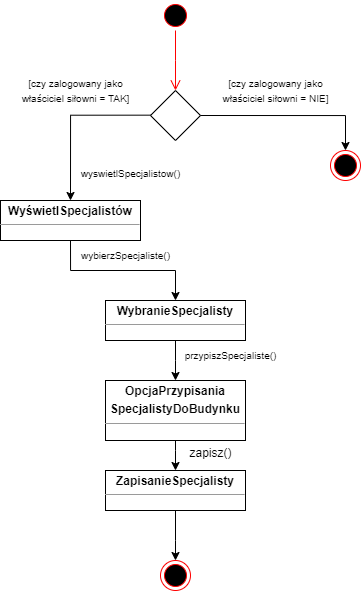
\includegraphics{diagrams/state/przypisz_specjaliste_budynku}}
{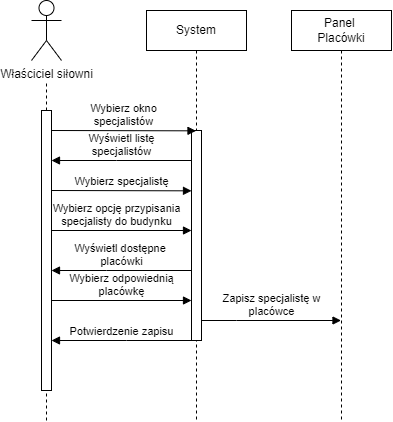
\includegraphics{diagrams/sequence/przypisz_speca_sekw}}

{Aktorzy biorący udział: Właściciel siłowni}

{~~~~~~~~Cel przypadku: Przypisanie specjalisty do danego budynku.}

{~~~~~~~~Warunki początkowe: Właściciel siłowni jest zalogowany w
systemie i ma dostęp do panelu właściciela siłowni.}

{~~~~~~~~Warunki końcowe: Specjalista przypisany do budynku.}

{~~~~~~~~Główny ciąg zdarzeń:}

\begin{enumerate}
\tightlist
\item
  {Właściciel siłowni otwiera okno ``Specjaliści''.}
\item
  {Użytkownik wybiera specjalistę docelowego.}
\item
  {Właściciel siłowni wybiera opcję ``Przypisz specjalistę do budynku''
  i wybiera z listy odpowiednią placówkę.}
\item
  {System zwraca informację o poprawnie wykonanej akcji.}
\end{enumerate}

{~~~~~~~~Alternatywny ciąg zdarzeń:}

\begin{itemize}
\tightlist
\item
  {~ Użytkownik nie posiada uprawnień właściciela siłowni.}
\end{itemize}

\begin{itemize}
\tightlist
\item
  {System wyświetla komunikat o braku uprawnień.}
\end{itemize}

\begin{itemize}
\tightlist
\item
  {Brak specjalistów}
\end{itemize}

\begin{itemize}
\tightlist
\item
  {System wyświetla komunikat o braku specjalistów.}
\end{itemize}

{}

{}

\begin{itemize}
\tightlist
\item
  {Istnieje tylko 1 placówka }
\end{itemize}

\begin{itemize}
\tightlist
\item
  {Specjalista jest automatycznie przypisywany do tej placówki.\\
  }
\end{itemize}

\begin{enumerate}
\setcounter{enumi}{18}
\tightlist
\item
  {Usuń specjalistę z budynku}
\end{enumerate}

{Aktorzy biorący udział: Właściciel siłowni}

{~~~~~~~~Cel przypadku: Usunięcie specjalisty z budynku.}

{~~~~~~~~Warunki początkowe: Właściciel siłowni jest zalogowany w
systemie i ma dostęp do panelu właściciela siłowni.}

{~~~~~~~~Warunki końcowe: Specjalista został usunięty z budynku.}

{~~~~~~~~Główny ciąg zdarzeń:}

\begin{enumerate}
\tightlist
\item
  {Właściciel siłowni otwiera okno ``Specjaliści''.}
\item
  {Użytkownik wybiera specjalistę docelowego.}
\item
  {Właściciel siłowni wybiera opcję ``Usuń specjalistę z budynku'' i
  potwierdza czynność.}
\item
  {System zwraca informację z potwierdzeniem czynności i wysyła prośbę
  do usuniętego specjalisty o dodatkowe potwierdzenie.}
\item
  {Specjalista jest usunięty z danego budynku, dane dla użytkowników są
  zaktualizowane.}
\end{enumerate}

{~~~~~~~~Alternatywny ciąg zdarzeń:}

\begin{itemize}
\tightlist
\item
  {~ Użytkownik nie posiada uprawnień właściciela siłowni.}
\end{itemize}

\begin{itemize}
\tightlist
\item
  {System wyświetla komunikat o braku uprawnień.}
\end{itemize}

\begin{itemize}
\tightlist
\item
  {Brak specjalistów}
\end{itemize}

\begin{itemize}
\tightlist
\item
  {System wyświetla komunikat o braku specjalistów.}
\end{itemize}

\begin{itemize}
\tightlist
\item
  {Właściciel siłowni nie potwierdził usunięcia specjalisty z budynku.}
\item
  {Specjalista nie potwierdził usunięcia z danego budynku.\\
  }
\end{itemize}

{}

{}

{}

{\includegraphics{diagrams/state/wypisz_użytkownika.png}}

\begin{enumerate}
\setcounter{enumi}{19}
\tightlist
\item
  {Wypisz użytkownika z treningu personalnego}
\end{enumerate}

{Aktorzy biorący udział: Właściciel siłowni}

{Cel przypadku: Usunięcie użytkownika z listy uczestników treningu
personalnego}

{Warunki początkowe: Właściciel siłowni ~jest zalogowany do systemu,
użytkownik jest zapisany na trening personalny}

{Warunki końcowe: Użytkownik zostaje usunięty z listy uczestników
treningu personalnego}

{Główny ciąg zdarzeń:}

\begin{enumerate}
\tightlist
\item
  {Właściciel siłowni loguje się do systemu.}
\item
  {Właściciel siłowni wybiera opcję "Zarządzanie treningami
  personalnymi".}
\item
  {System wyświetla listę zapisanych na trening personalny
  użytkowników.}
\item
  {Właściciel siłowni wybiera użytkownika, którego chce usunąć z
  treningu personalnego.}
\item
  {System wyświetla szczegóły zapisu użytkownika na trening personalny.}
\item
  {Właściciel siłowni wybiera opcję "Usuń użytkownika".}
\item
  {System usuwa użytkownika z listy uczestników treningu personalnego i
  wyświetla stosowną informację.}
\item
  {Właściciel siłowni kończy procedurę i wylogowuje się z systemu.}
\end{enumerate}

{Alternatywne ciągi zdarzeń:}

\begin{itemize}
\tightlist
\item
  {W przypadku, gdy użytkownik nie jest zapisany na trening personalny,
  system wyświetli stosowną informację.}
\item
  {W przypadku, gdy użytkownik ma już opłacony trening personalny,
  system zapyta, czy chce zwrócić pieniądze użytkownikowi lub przesunąć
  go na inny trening personalny.}
\end{itemize}

{}

{}

\begin{enumerate}
\setcounter{enumi}{20}
\tightlist
\item
  {Wypisz użytkownika z treningu grupowego}
\end{enumerate}

{Aktorzy biorący udział: Właściciel siłowni}

{Cel przypadku: Usunięcie użytkownika z rezerwacji na trening grupowy.}

{Warunki początkowe: Użytkownik jest zarejestrowany na trening grupowy,
trening grupowy jest zaplanowany na konkretny dzień i godzinę.}

{Warunki końcowe: Użytkownik został usunięty z rezerwacji na trening
grupowy.}

{Główny ciąg zdarzeń:}

\begin{enumerate}
\tightlist
\item
  {Właściciel siłowni loguje się do systemu.}
\item
  {Właściciel siłowni znajduje użytkownika na liście uczestników
  treningu grupowego.}
\item
  {Właściciel siłowni usuwa użytkownika z rezerwacji na trening
  grupowy.}
\item
  {System wyświetla komunikat potwierdzający usunięcie użytkownika.}
\end{enumerate}

{Alternatywne ciągi zdarzeń:}

\begin{itemize}
\tightlist
\item
  {Jeśli użytkownik nie został znaleziony na liście uczestników treningu
  grupowego, system wyświetla komunikat o błędzie i prosi o wprowadzenie
  poprawnych danych.}
\item
  {Jeśli trening grupowy został odwołany lub zmieniony, system wyświetla
  komunikat informujący o zmianach i proponuje przypisanie użytkownika
  do innego treningu grupowego.}
\end{itemize}

{}

{}

{}

\begin{enumerate}
\setcounter{enumi}{21}
\tightlist
\item
  {Wypisz użytkownika z rehabilitacji}
\end{enumerate}

{Aktorzy biorący udział: Właściciel siłowni}

{Cel przypadku: Usunięcie użytkownika z listy uczestników rehabilitacji}

{Warunki początkowe: Właściciel siłowni jest zalogowany do systemu i
posiada uprawnienia do zarządzania rehabilitacją}

{Warunki końcowe: Użytkownik zostaje usunięty z listy uczestników
rehabilitacji}

{Główny ciąg zdarzeń:}

\begin{enumerate}
\tightlist
\item
  {Właściciel siłowni wybiera moduł zarządzania rehabilitacją}
\item
  {Właściciel siłowni wyszukuje użytkownika, którego chce usunąć z listy
  uczestników rehabilitacji}
\item
  {Właściciel siłowni otwiera kartę użytkownika i wybiera opcję "Usuń
  użytkownika z listy rehabilitacji"}
\item
  {System wyświetla komunikat potwierdzający operację usuwania}
\item
  {Właściciel siłowni potwierdza chęć usunięcia użytkownika z listy
  uczestników rehabilitacji}
\item
  {System usuwa użytkownika z listy uczestników rehabilitacji}
\item
  {System wyświetla potwierdzenie usunięcia użytkownika z listy
  uczestników rehabilitacji}
\end{enumerate}

{Alternatywne ciągi zdarzeń:}

\begin{itemize}
\tightlist
\item
  {Jeśli użytkownik nie jest obecny na liście uczestników rehabilitacji,
  to właściciel siłowni otrzymuje komunikat informujący o tym fakcie.}
\item
  {Jeśli wystąpią problemy z usunięciem użytkownika z listy uczestników
  rehabilitacji, system wyświetli komunikat z informacją o błędzie.}
\end{itemize}

{}

{}

\begin{enumerate}
\setcounter{enumi}{22}
\tightlist
\item
  {Wypisz użytkownika z wizyty u dietetyka}
\end{enumerate}

{Aktorzy biorący udział: Właściciel siłowni}

{Cel przypadku: Usunięcie użytkownika z listy zarejestrowanych na wizytę
u dietetyka}

{Warunki początkowe: Właściciel siłowni jest zalogowany do systemu,
użytkownik jest zarejestrowany na wizytę u dietetyka}

{Warunki końcowe: Użytkownik zostaje usunięty z listy zarejestrowanych
na wizytę u dietetyka}

{Główny ciąg zdarzeń:}

\begin{enumerate}
\tightlist
\item
  {Właściciel siłowni wybiera opcję zarządzania wizytami u dietetyka.}
\item
  {System wyświetla listę użytkowników zarejestrowanych na wizytę u
  dietetyka.}
\item
  {Właściciel siłowni wybiera użytkownika, którego chce wypisać z
  wizyty.}
\item
  {System wyświetla potwierdzenie usunięcia użytkownika z listy
  zarejestrowanych na wizytę.}
\item
  {Właściciel siłowni potwierdza usunięcie użytkownika.}
\item
  {System usuwa użytkownika z listy zarejestrowanych na wizytę u
  dietetyka.}
\item
  {System wyświetla potwierdzenie usunięcia użytkownika z listy.}
\end{enumerate}

{Alternatywne ciągi zdarzeń:}

\begin{itemize}
\tightlist
\item
  {~Jeśli właściciel siłowni nie może znaleźć użytkownika na liście
  zarejestrowanych na wizytę u dietetyka, to system wyświetla komunikat
  informujący o tym fakcie.}
\end{itemize}

{}

{}

{}

{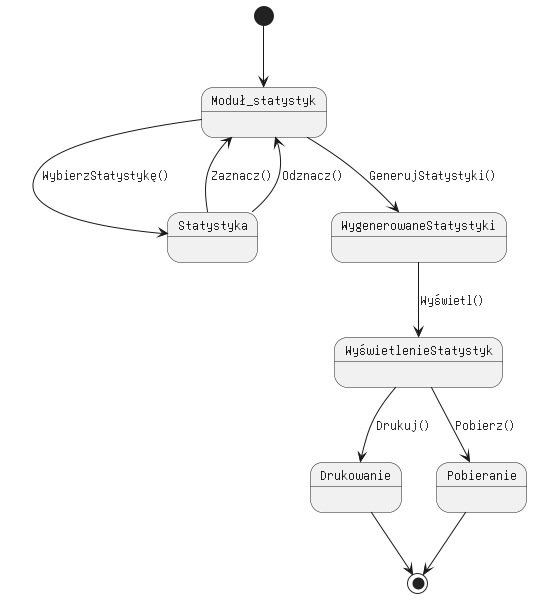
\includegraphics{diagrams/state/wygeneruj_statystyki.png}}

\begin{enumerate}
\setcounter{enumi}{23}
\tightlist
\item
  {Wygeneruj statystyki}
\end{enumerate}

{Aktorzy biorący udział: Właściciel siłowni}

{Cel przypadku: Wygenerowanie różnych statystyk dotyczących działalności
siłowni, takich jak przychody, ilość użytkowników, popularność zajęć,
wykorzystanie sprzętu.}

{Warunki początkowe: Właściciel siłowni jest zalogowany do systemu
zarządzania siłownią.}

{Warunki końcowe: Wygenerowanie i wyświetlenie statystyk dotyczących
działalności siłowni.}

{Główny ciąg zdarzeń:}

\begin{enumerate}
\tightlist
\item
  {Właściciel siłowni wybiera moduł zarządzania finansami.}
\item
  {Właściciel siłowni wybiera opcję "Wygeneruj statystyki".}
\item
  {System wyświetla różne opcje statystyk do wyboru, takie jak
  przychody, ilość użytkowników, popularność zajęć itp.}
\item
  {Właściciel siłowni wybiera interesującą go opcję statystyk.}
\item
  {System generuje statystyki i wyświetla je na ekranie.}
\item
  {Właściciel siłowni może wydrukować lub pobrać statystyki w formacie
  pliku.}
\end{enumerate}

{Alternatywne ciągi zdarzeń:}

\begin{itemize}
\tightlist
\item
  {Jeśli system nie może wygenerować statystyk z powodu braku danych,
  wyświetlany jest komunikat informujący o tym fakcie. Właściciel
  siłowni może wtedy zdecydować się na inne statystyki lub wykonać
  czynności, które umożliwią generowanie wybranych statystyk.}
\end{itemize}